\documentclass{article}
\usepackage{graphicx}
\graphicspath{{./figure/}}  % папки с картинками

\begin{document}

\begin{titlepage}
	
	\begin{center}
		
		\vspace{1cm}

		{\Huge \textsc{U s e r' s \, \, G u i d e}}
		
		
		\vspace{1cm}
		\hrulefill
		\vspace{1cm}
		
		{\Huge \textbf{GUI4DFT \, \, 1.3}}
		
		\vspace{1cm}
		\hrulefill
		\vspace{0.5cm}
		
		%{\Large \printdate}
		
		\vspace{1.5cm}
		{\Large https://github.com/sozykinsa/GUI4dft}
		
		\vspace{2.5cm}
		%Steering Committee:
		\vspace{1.0cm}
		
		\begin{tabular}{ll}
			
			Sergey Sozykin  \\  %&
			\textit{South Ural State University, Chelabinsk, Russia} \\
			
			% ...
						
		\end{tabular}
		
	\end{center}
	
\end{titlepage}

	
	
\section{About GUI4DFT program}

The Graphical User Interface for Density Functional Theory (GUI4dft) allows the user to work directly with SIESTA input and output files and prepare manuscript-quality figures of the atomic structure and properties such as three-dimensional charge density distributions, DOS, PDOS, and band structure.

It is a SIESTA oriented cross-platform program. The program was tested in Windows, Mac OS and Ubuntu operating systems.

The main window of the program is shown in Fig. \ref{fig:mainwindow}.

\begin{figure}[h!]
	\centering
	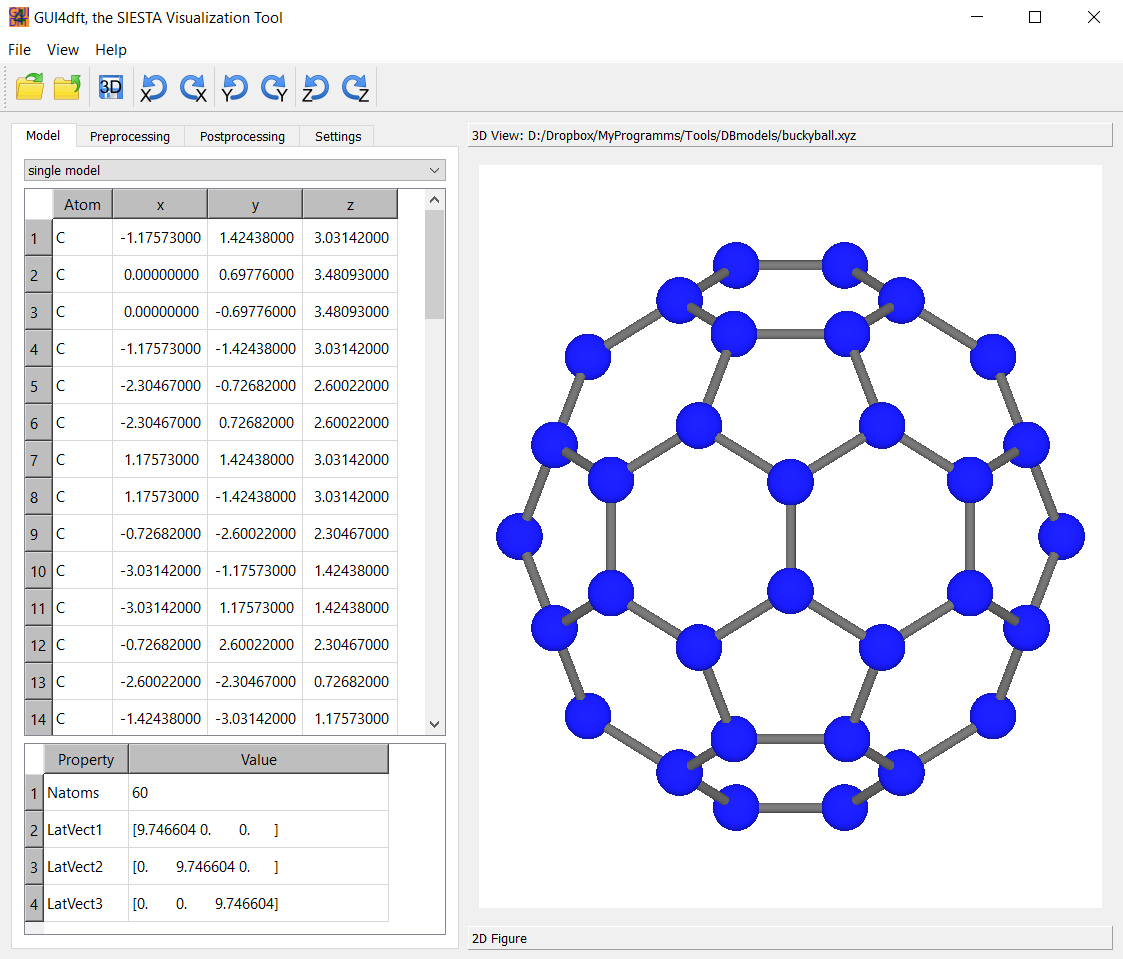
\includegraphics[width=5.0in]{mainwindow}
	\caption{The main window of GUI4dft}
	\label{fig:mainwindow}
\end{figure}

\section{Installation}

GUI4DFT program is written in Python 3 (version >= 3.4). I recommend using the python distribution kit from the https://www.python.org/ website. GUI4DFT has some dependences. To install the necessary modules, run in the terminal (in the folder where the requirements.txt file is located):

pip3 install -r ./requirements.txt

You have to set the variable QT\_API. In linux you can add this line to the bashrc file:\\
export QT\_API=pyside2 \\
In Windows open the Start Search, type in “env”, and choose “Edit the system environment variables”. Click the “Environment Variables...” button. Add new variable “QT\_API” with value “pyside2”. 

To run the program, type

python3 gui4dft.py
	
\section{GUI}

The program combines a set of tools for preparing an input file for a SIESTA package and for post-processing of calculation results. The main window of the program consists of several parts (see Fig.\ref{fig:mainwindow}). On the left side of the screen are tabs Model, Preprocessing, Postprocessing and Settings. On the right side of the screen, 3D models and graphs are displayed.

Using the <<File>> button located on the top panel, user can open a file with information about the atomic structure (*.fdf, SystemLabel.ANI, SystemLabel.STRUCT\_OUT, SystemLabel.XSF, SystemLabel.cube, *.out).

The values of the drop-down menu <<Open>> and <<Export>> are duplicated just below the folder images. To the right is the button for saving the contents of the <<3D View>> tab and the buttons for controlling the rotation of the 3D model of the atomic structure.

The atomic structure is displayed in the <<3D View>> tab, the coordinates of atoms corresponding to the model and the size of the calculation cell are displayed on the <<Model>> tab.

The <<View>> button allows user to customize the presentation of the 3D model (perspective and display of cell borders).

	
\subsection{Model}

This tab displays general information about the atomic model: coordinates of atoms, vectors of a unit cell. If the file you are viewing contains information about several steps of atomic structure optimization, you can view each of them. The available atomic structures are shown in the drop-down list at the top of the section.

\subsection{Preprocessing}

Using the Preprocessing tab, user can set the structure of the model and generate an *.fdf file. It is possible to generate the following structures: single-layer nanotube, graphene; model consisting of two parts; model with electrodes.

\subsubsection{Create}

This tab allows you to create models of carbon nanotubes, graphene, as well as combine electrode models with the model under study.

\textbf{Graphene}

The size of the created graphene model is set by two integers defining one of the graphene boundaries and the length of the model in the direction perpendicular to this boundary.

\textbf{SWNT}

The program allows you to create models of nanotubes with open ends (any chirality indices), with one or two closed ends (only for nanotubes (6,6) and (10,0)). When creating models of nanotubes with closed ends, it is required to indicate the rotation angles for the caps and the distance from the caps to the nanotube atoms. The user can specify the length of the model in angstroms or in the unit cell length.

After setting the parameters, user must click on <<Create>>, the result will be displayed in the <<3D-View>> window (see Fig. \ref{fig:createswnt})

\begin{figure}[h!]
	\centering
	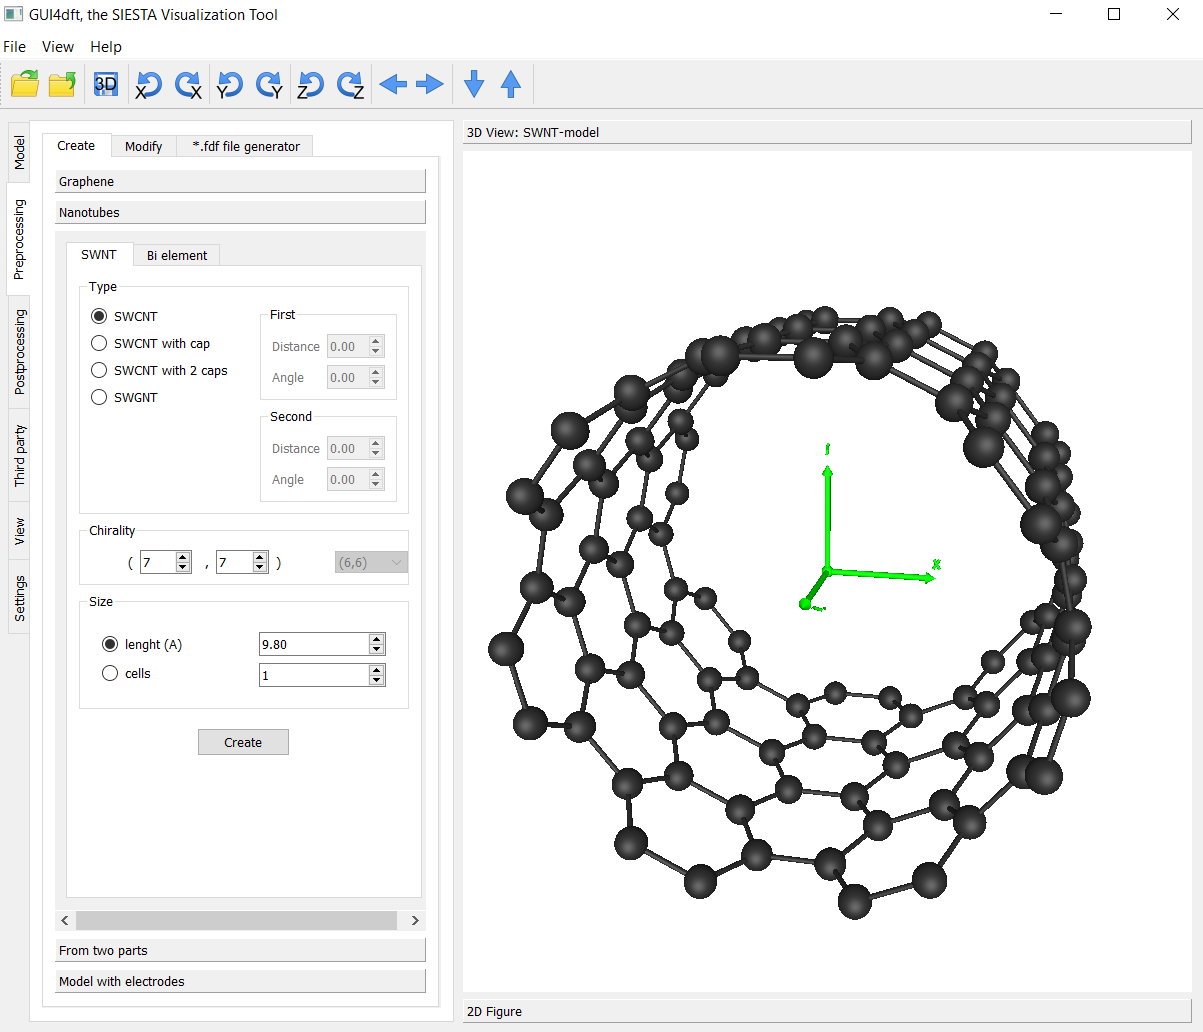
\includegraphics[width=10.0cm]{create_swnt}
	\caption{Generation of a single-walled nanotube}
	\label{fig:createswnt}
\end{figure}

In the next tab, user can create a nanotube consisting of two elements: B and N or B and C (selection in the drop-down list). User can also set the type of nanotube (armchair or zigzag), chirality and length (see Fig. \ref{fig:create_bint}).

\begin{figure}[h!]
	\centering
	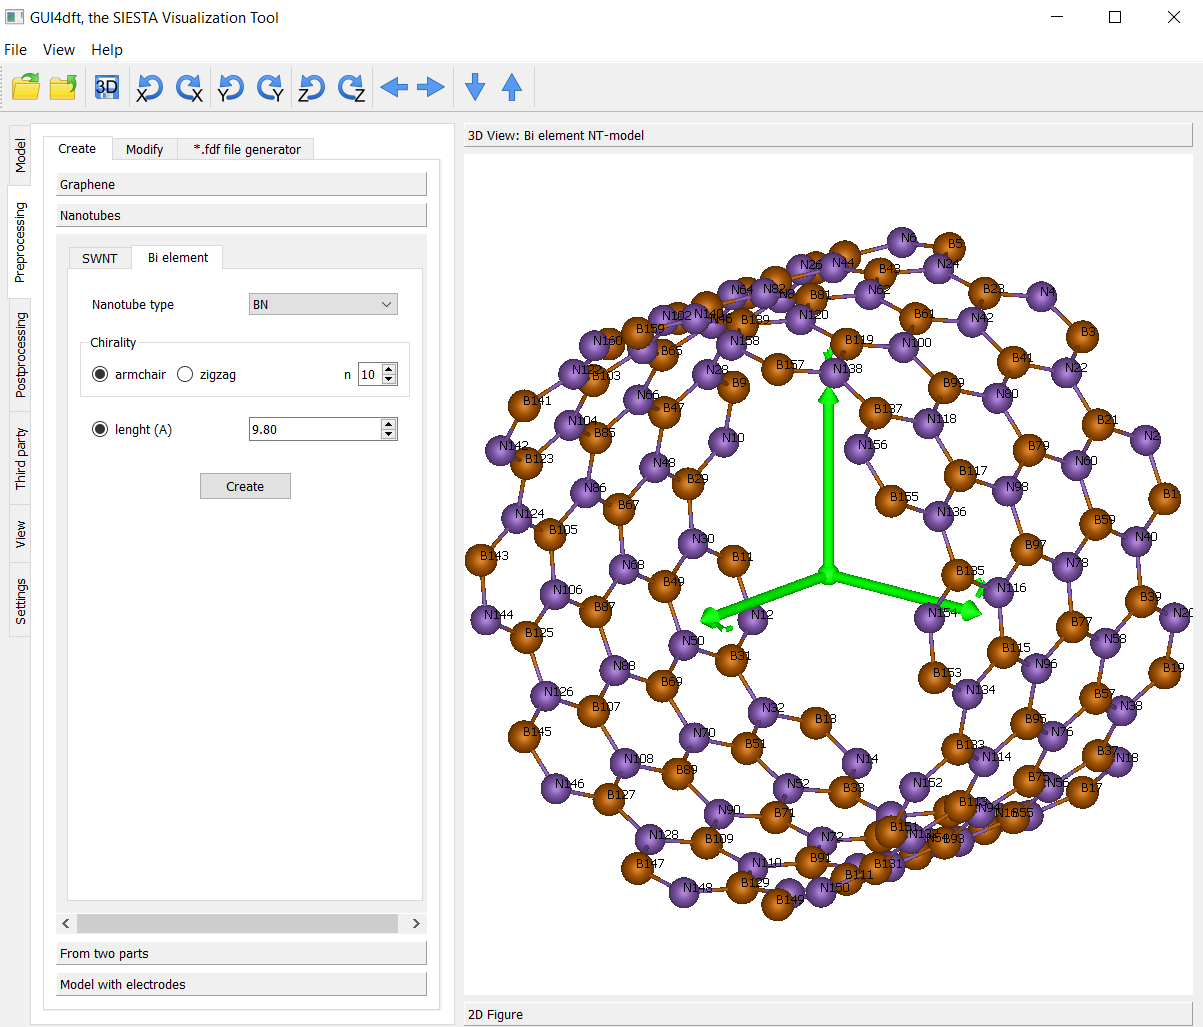
\includegraphics[width=10.0cm]{create_bint}
	\caption{Nanotube consisting of two elements}
	\label{fig:create_bint}
\end{figure}

\textbf{From two parts}

For a model that consists of two parts, user need to load two separate input files, set the angle of rotation and the center of mass for each, then click <<Create>>.

\textbf{Model with electrodes}

To study the transport properties, it is necessary to prepare a model consisting of two electrodes and the scattering area. The graphical interface allows you to specify *.fdf files containing a description of the atomic structure of each of the three parts. The user can set the distance from the electrodes to the investigated fragment, as well as the angle of rotation of the investigated fragment. Both for the electrodes and for the region of rotation, user can set a shift in coordinates.

\subsubsection{Modify}

This tab contains tools for modifying the viewed atomic structure and preparing the input file for the SIESTA package.

An atom can be selected by clicking on the corresponding model atom (the <<allow atom selection>> must be checked in the settings); after that, it can be removed or the coordinates changed. User can add your own atom by selecting an element, specifying coordinates, and clicking <<Add>>.

The <<Cell>> tab allows the user to set the length of the translation vectors.

In the <<Fill Space>> tab, the user can search for various configurations of a given number of atoms in a given cylindrical volume. Available parameters: the number of atoms, their charge, the value of the <<delta>> parameter, the radius of the cylinder and its height.
Using the <<Grow model>> tab, the model can be translated along the axes.

Using the “Rotate model” tab, respectively, the user can rotate the model by a certain degree relative to a given axis around the origin or center of mass, or twist the model along the z axis by a given degree (<<Twist (z-axis)>> block).

\subsubsection{*.fdf file generator}

This tab allows you to prepare an input file for the SIESTA package. If the atomic system displayed in the program is obtained from a fdf file or the output stream of the SIESTA package, the generated text is ready for launch. Otherwise, only information related to the atomic structure is available.

The formats for the representation of translation vectors and atomic coordinates are configured on the tab described in the section \ref{settingsmode}.

The text is created by clicking the Generate button. This text can be edited directly in the program or saved to a file by clicking on the Save button.


\subsection{Postprocessing}

This tab is responsible for post-processing SIESTA output files.

\subsubsection{Electronic properties}

Note that to work with the SystemLabel.DOS, SystemLabel.pdos, SystemLabel.bands files, user need to open the SystemLabel.out file located in the same folder.


\textbf{Band structure}

To get a band structure graph, in the “Band structure” tab, click the “parse BANDS” button. When you click on the "parse BANDS" button, a text file indicated in the text field above the button (it is filled in automatically) is analyzed and then click “plot BANDS” to plot the graph. 

The user can also customize the display of the graph: select k-range and Energy range, display the Fermi level (check the box next to <<show>> in the <<Fermi energy>> field). It is possible to build different graphs for the spin of different directions. Below user can set the name of the graph and labels for the axes. At the very bottom of the tab, the width of the direct and indirect bandgap is displayed.

The resulting graph will be displayed in the «2D Figure» tab, as shown in Fig. \ref{fig:postbands}.


\textbf{DOS}

To build the density of states (DOS), user need to go to the DOS tab. The table (see Fig. \ref{fig:postdos}) will display the SystemLabel.DOS output file used for analysis and the corresponding value of the Fermi energy. Below are checkboxes for setting the display of the Fermi level, drawing lines for both directions of the spin at the same time, as well as inverting these positions (shown in Fig. \ref{fig:postdos} by lines of different colors).

\begin{figure}[h!]
	\centering
	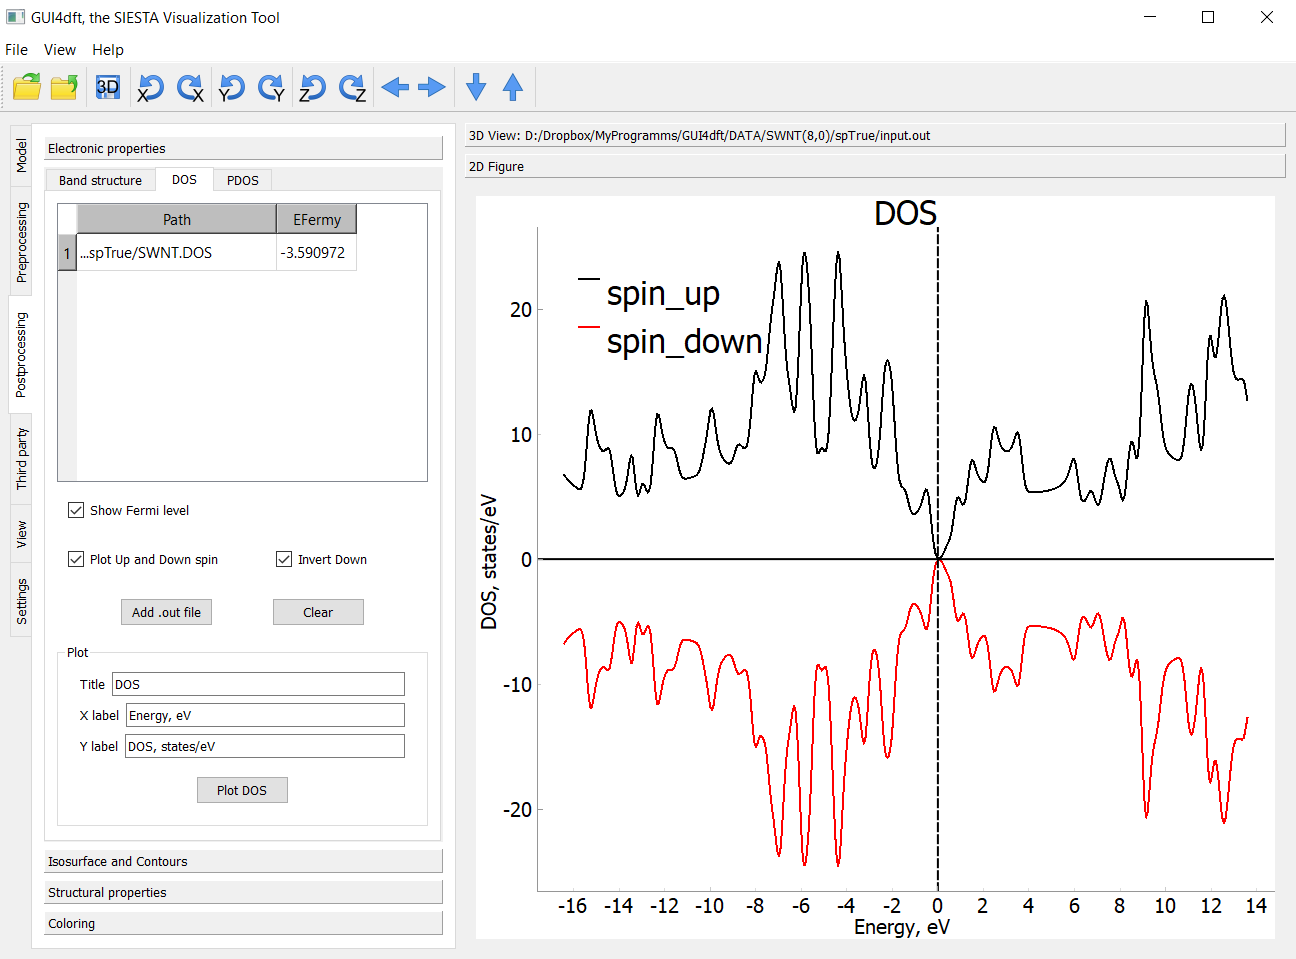
\includegraphics[width=12.0cm]{post_dos}
	\caption{Formation of the density of electronic states}
	\label{fig:postdos}
\end{figure}

Click <<Plot DOS>> to display the graph. To add another output file, click <<Add .out file>>. The new SystemLabel.DOS file will be displayed in the table as a new line - by clicking on it, user select a file for further work.

Below is a block for setting the name of the chart and axes.


\textbf{PDOS}

Plotting the density of partial electronic states begins with the «PDOS» tab. In the <<Indexes>> tab, user need to select from the drop-down list the indices of which atoms user want to consider: all atoms selected on the 3D model or entered in the field below. 

In the <<Species>> tab, the selection of structure elements for which the density will be built is carried out, similarly to indices.

Using the other tabs, user can select the orbitals for which the density will be built. To select an orbital, the tabs <<n>>, <<m>>, <<l>> and <<zeta>> are provided, inside which there are checkboxes.

Below are checkboxes for setting the display of spin and Fermi energy.
After completing the display settings, user must enter the designation for the density of partial electronic states in the field and click <<plot single PDOS and add to list>>. The configured DOS will also be added to the list below, and the corresponding graph will be displayed in the <<2D-Figure>> window.

By highlighting the necessary data in this list, after pressing “plot selected DOS”, user can build a graph with the simultaneous presentation of several densities of partial electronic states.

\subsubsection{Isosurface and Contours}

Files with *.XSF and *.cube extensions are accepted as an input file for generating isosurfaces and contours; they must be located in the same folder as the SystemLabel.out file. 

\textbf{Data 1}

The “Data 1” tab displays the files of the required extension found in the folder. To work with the desired file, select it and click <<Parse>>. The file structure will be displayed below in tree form. After selecting the desired data, user must click <<Load Data>> to load the data and the resulting range of data values in the file will be displayed under the button.

\textbf{Data 2}

This tab is intended for calculating the sum or difference of two data sets with the possibility of further visualization or export to a file. If the operation has been performed, further actions are performed on the result of this operation.

Important: an operation with data is allowed only if the dimensions of the grids coincide.


\textbf{Isosurface}

To display the values selected in the future, check the <<Show>> checkbox. Values are added to the field with the table using the <<Add>> button opposite the field for entering values. To delete a value from the table, use the <<Delete>> button; to display the isosurface in the <<3D-View>> window, click the <<Plot>> button.

By default, the isosurface color corresponds to the color scheme described in the tab <<View>> $\rightarrow$ <<Color>> $\rightarrow$ <<Other Colors>>. In the table, the user can adjust the color for the value (double click on the cell in the <<Value>> column) and transparency (the <<Transparency>> column). 

\textbf{Contours}

In contours, the color of the lines corresponds to the value of the physical quantity, for planes, the color of each pixel corresponds to the value of the physical quantity at a given point, in the plane + contours mode, contours appear near the plane. Visualization can be carried out for one, two or three planes (XY, XZ, YZ). For each of them, the user can independently set the position using the slider and the number of contours in the <<levels>> field. To display the selected contour or plane, check the corresponding checkbox <<show>> and press the <<Plot>> button.

\subsubsection{Structural properties}

\textbf{Bonds}

In the <<Bonds>> section, work with interatomic bonds is carried out. After clicking on the <<Get bonds>> button, a list of all bonds and their lengths will appear in the table. Below user can select from the drop-down list what type of relationships to use for plotting diagrams (between which elements). The average value of the interatomic bond is also shown. There is also a field for setting the number of columns of the histogram of the distribution of bond lengths and the <<Plot histogram>> button for plotting a histogram in the <<2D Figure>> window.

\textbf{Cell parameter}

This tab allows you to determine the equilibrium volume (or the translation along one of the axes) from a series of calculations with different parameters of the unit cell. The approximation can be carried out using the equations of Murnaghan, Birch-Murnaghan, or quadratic dependence.

In the <<Cell paramerter>> section, the equilibrium cell parameter is visualized. In the drop-down list, the user selects the Murnagam and Birch-Murnagam equations of state or quadratic approximation, and the required parameter is selected in the list to the right. The table below shows the parameters obtained from the output file. To add files, click <<Add File>>. User can also enter parameters manually: click <<Add Row>> to add an empty row and then double-click on an empty cell to enter data. To delete the selected row, click <<Delete Selected>>. To import a finished table, click <<Import>>. To start the optimization, user must click <<Optimize>>. The optimal value of the selected parameter and the corresponding values of the other parameters will appear below. The graph will appear in the <<2D Figure>> field.

\textbf{Selection history}

The <<Selection history>> tab displays the history of selected atoms, the number of the currently selected atom, its element, as well as the distance between the last two selected atoms and the angle between the last three selected. Below there is a field for calculating the distance between any two atoms: enter their numbers and click <<Get>>.

\textbf{Voronoi}

This tab allows you to plot a Voronoi polyhedron for a selected atom.

The <<Voronoi>> tab sets the maximum distance for the Voronoi polyhedron for the selected atom. To plot a polyhedron on a 3D model, click on <<Plot>>. The tab below will display the number of the atom and the volume of the polyhedron.

\subsubsection{Coloring}

This tab allows you to color the atoms in accordance with their property (Milliken, Voronoi or Hirschfield charges). This option is only available for equilibrium configuration and if the corresponding property has been calculated.

To change the transparency of selected atoms, check the <<Activate fragment selection mode>> checkbox and select transparency in the field below. The selected atoms will be displayed below the field.

To apply changes to atoms with a coordinate belonging to a certain range, enter the minimum and maximum values for the desired coordinate in the fields below and click <<change status>>.

Both change modes can be applied at the same time.

To cancel the changes, click <<clear>> at the bottom of the tab.



\subsection{View}

\subsubsection{View 3D}

The <<View 3D>> tab allows user to set the visibility of atoms, cells, atom numbers and coordinate axes using checkboxes. Below are the fields for setting the width of the contours and the viewing angle in perspective mode. In the <<Bonds>> block, the visibility of interatomic bonds, their width and color (by default or matching the color of atoms) are configured. Below is a field for obtaining the value of the length of the connection between various elements of the system.

\subsubsection{View 2D}

The <<View 2D>> tab is intended for setting the color of the text on the graphs (set as three numbers of the RGB color scheme). Below is a block for setting font sizes for graph titles, their axes and symbols. In addition, it is possible to adjust the width of the lines. To apply the changes, click <<Apply style>>.

\subsubsection{Colors \label{colorsisos}}

The <<Colors>> tab is responsible for the color scheme of atoms: above the list of elements there are radio buttons for choosing from three schemes. The default scheme (manual) is available for editing by double-clicking on the desired element. In the <<Other Colors>> section, the background color, the default color of links, cell borders, axes, and the Voronoi polyhedron are configured.

Below user can select a color scheme for contoured planes from the drop-down list. An example of the selected color scheme will be located below the drop-down list. User can also select the scale (linear or logarithmic), change the outline color, and set a fixed range of colors.


\subsection{Settings \label{settingsmode}}

The <<Settings>> tab contains the following checkboxes: get only the optimal structure, analyze the properties of an atom, allow the selection of atoms, allow the model to be moved. The drop-down lists below select preferred units (boron or angstrom), atomic coordinates, and preference for using a lattice parameter or lattice vectors.


\textbf{Get only optimal structures}. If this option is selected, the program displays information only about the equilibrium model from the SIESTA output file.


\textbf{Parse atomic properties}. If this option is selected and the output file contains the charges of atoms (Milliken, Voronoi and Hirshfeld), these charges will be displayed in the Postprocessing $\to$ Structural properties $\to$ Selection history tab and can be used to color atoms in the system (Postprocessing $\to$ View).


\textbf{Allow atom selection}. If this option is selected, atoms can be selected using the mouse.


\textbf{Preferred coordinates}. This option defines the way of specifying coordinates in the *.fdf file (Postprocessing $\to$ Modify $\to$ *.fdf file generator): "Zmatrix Cartesian" or "Fractional".


\textbf{Preferred lattice}. This option defines the way of specifying the elementary cell in the *.fdf file.


\subsection{Working with graphs}

Moving away or zooming in on the chart is done with the mouse wheel or by selecting a fragment of the chart with the left mouse button pressed. To reset the scale, right-click on the chart and select <<View All>> from the list.

To set up the display of axes: right-click on the graph and select the desired axis in the list (Fig. \ref{fig:graph1}).


\begin{figure}[h!]
	\centering
	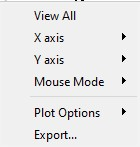
\includegraphics[width=5.0cm]{graph1}
	\caption{Graph editing menu}
	\label{fig:graph1}
\end{figure}

For the axis, user can select a range of scale values (first line) or set a value in percent (second line) (Fig. \ref{fig:graph2}). If the value is specified as a percentage, in the checkboxes below, user can set the auto-scaling to take into account only the data visible relative to the axis (Visible Data Only). With the <<Auto Pan Only>> checkbox checked; the axis will be shifted to the middle of the considered data (without changing the scale step). Below user can configure scale inversion and enable/disable mouse control (zoom and pan) for the axis.

\begin{figure}[h!]
	\centering
	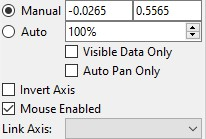
\includegraphics[width=5.0cm]{graph2}
	\caption{Axis appearance editing submenu}
	\label{fig:graph2}
\end{figure}

The <<Mouse mode>> menu item allows the user to select the mouse control mode: 1 or 3 buttons.

In the lower menu block, there are buttons for calling the submenu of chart options (displaying a grid and data markers, transformation, reducing resolution, finding average values) and a button for exporting a 2D figure.

\section{Conclusion}
All comments on the work of the program, please send to the email address sozykinsa@susu.ru
	
\bibliography{bibdatabase}
	
\end{document}